% \clearpage
\phantomsection% ensures hyperref works properly
\addcontentsline{toc}{section}{\hspace*{-1em}Приложение А (обязательное) Отчет о проверке на заимствование}\par

\normalsize
\begin{center}
  \textbf{ПРИЛОЖЕНИЕ А} \\
  \textbf{(обязательное)} \\
  \textbf{Отчет о проверке на заимствование}
\end{center}

% \clearpage
\renewcommand{\thefigure}{А.\arabic{figure}} % Нумерация рисунков в виде А.1
\setcounter{figure}{0}                       % Сброс счётчика рисунков (по желанию)

\insertfigure{pl}{pic/pl.png}{Результат проверки на плагиат}{14.0cm}

\begin{flushright}
  \begin{minipage}{0.5\textwidth}
    \raggedright
    \underline{\hspace*{3.7cm}} Кривальцевич Е.А.
  \end{minipage}
\end{flushright}

% Установка размера страницы A3 в альбомной ориентации
% \pdfpagewidth=420mm
% \pdfpageheight=297mm

% \thispagestyle{empty} % Убрать номер страницы

% Вставка листа A3
% 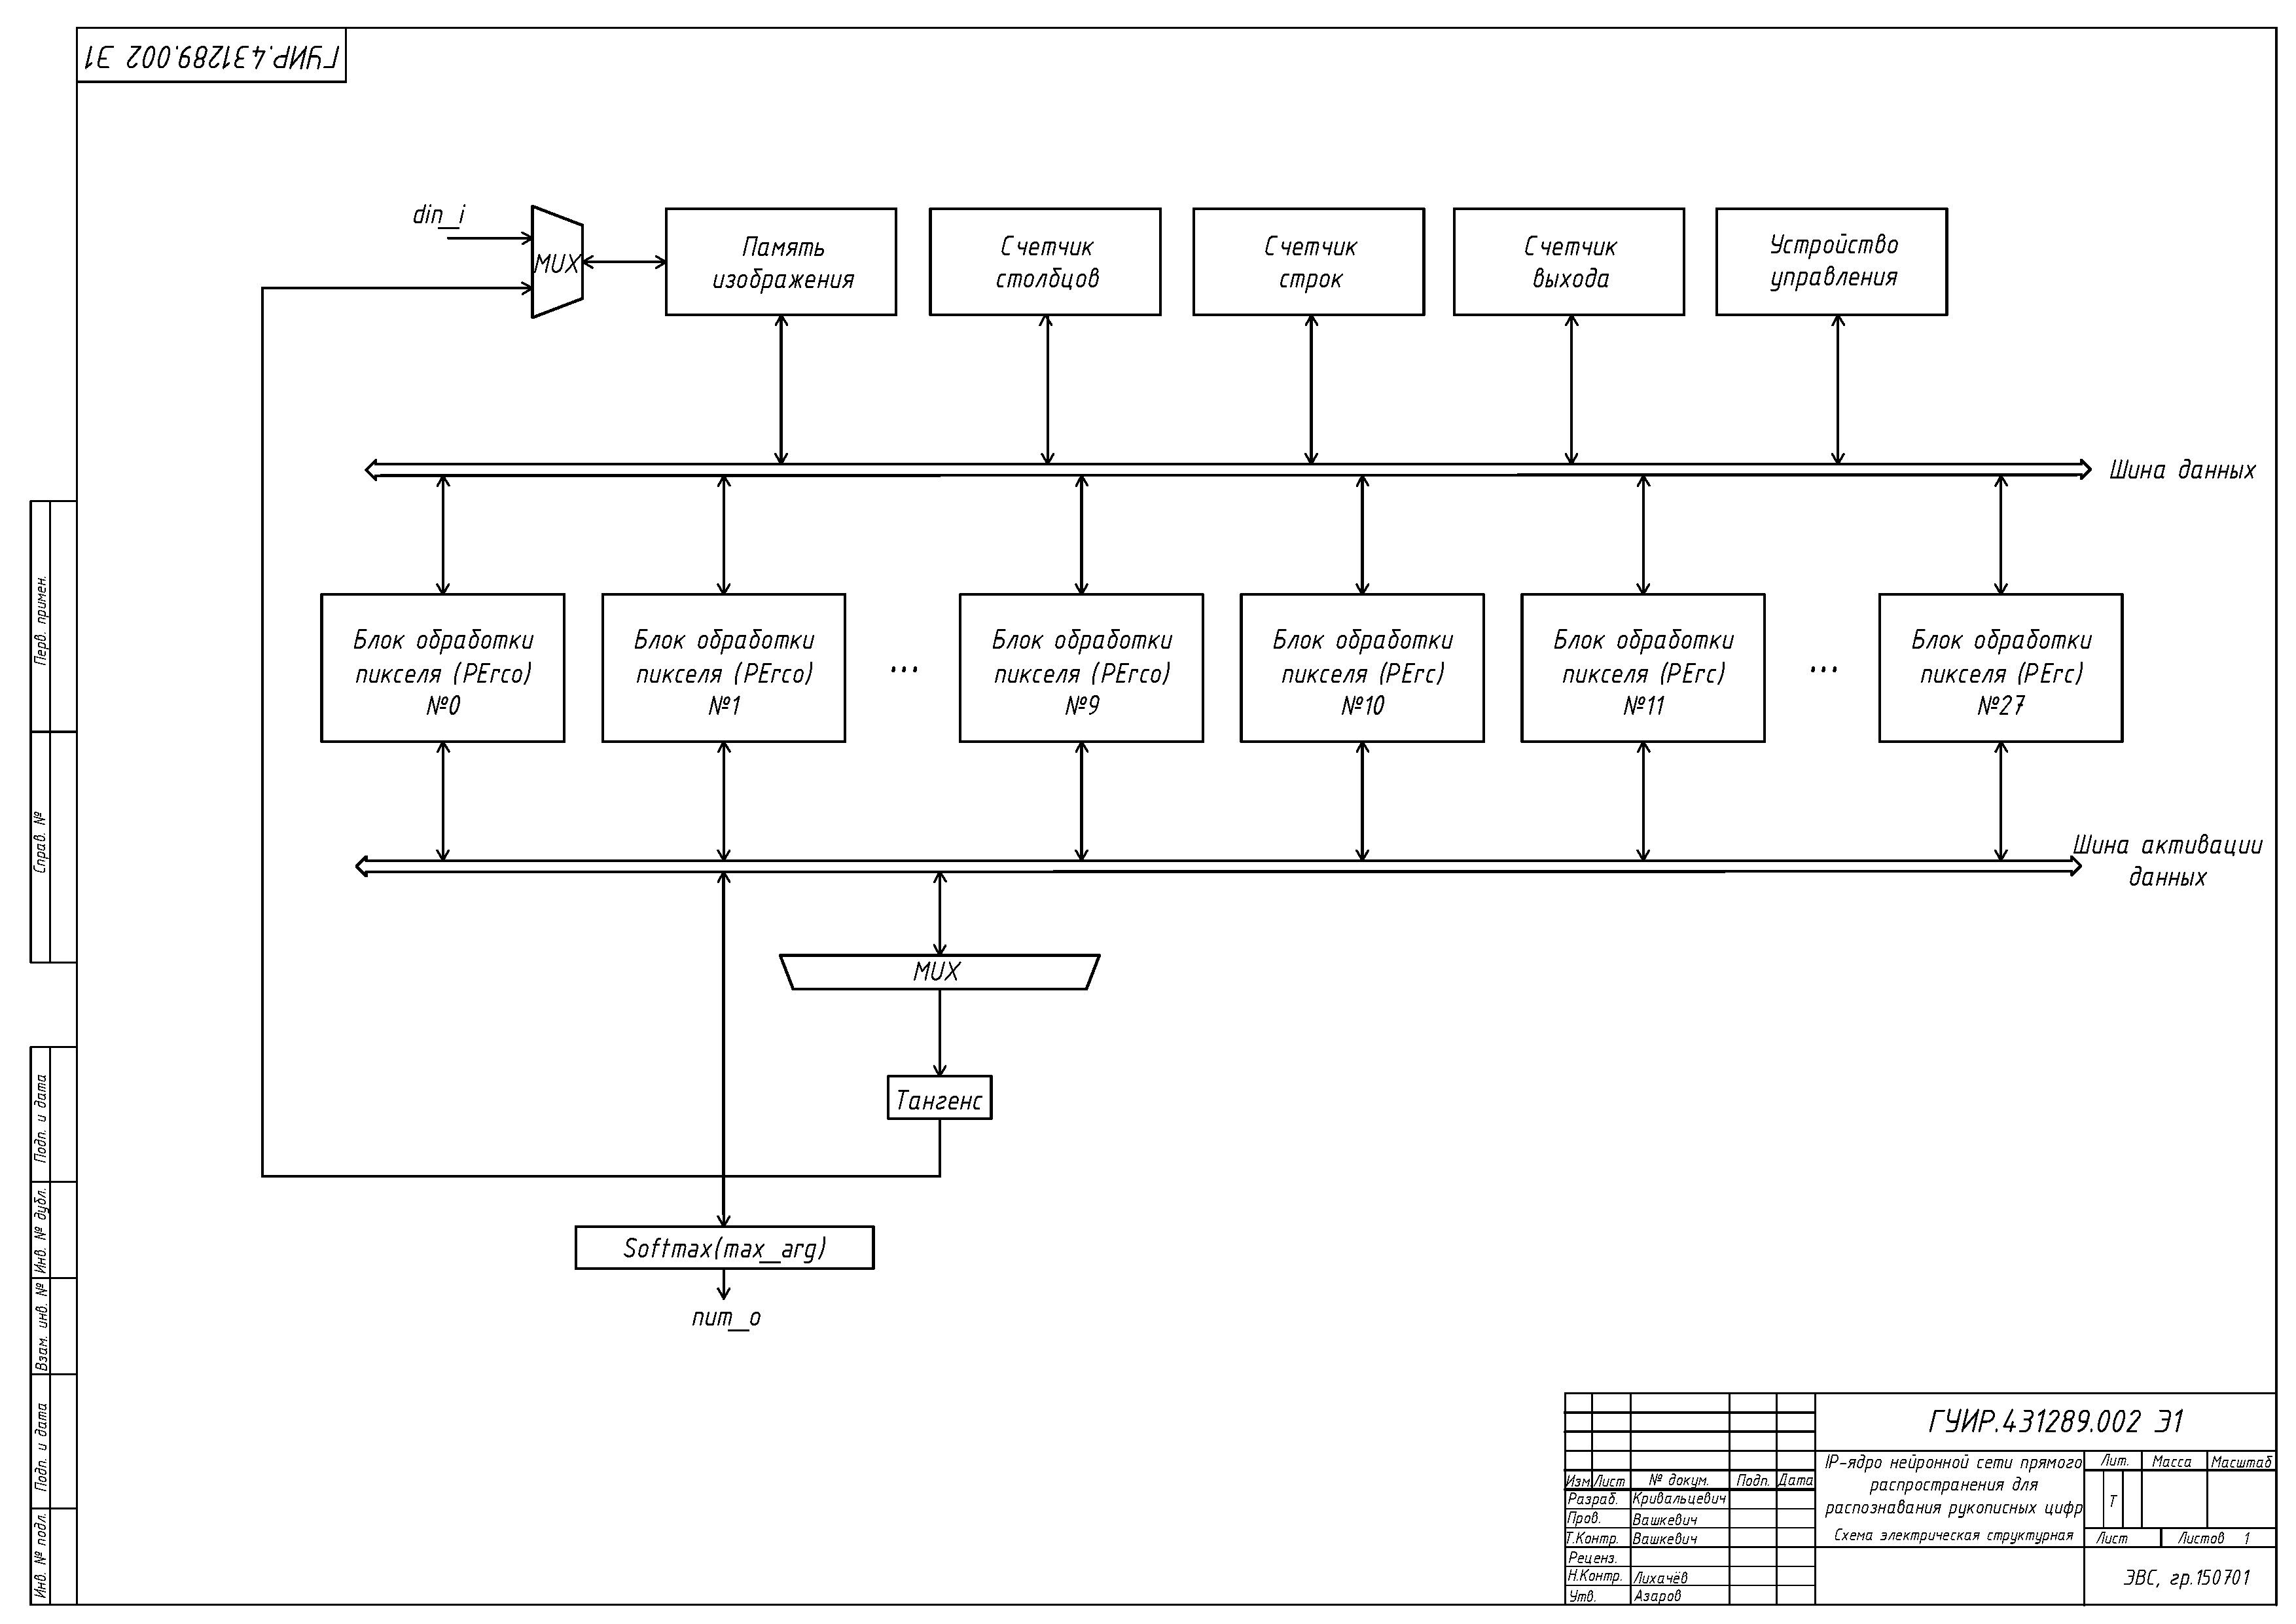
\includepdf[pages=-, pagecommand={}, fitpaper, offset=0 0]{STRUCT.pdf}

% Восстановление размера страницы A4
\pdfpagewidth=210mm
\pdfpageheight=297mm

\clearpage
